\documentclass[11pt]{article}
\usepackage{../EllioStyle}
\usepackage{listings}
\usepackage{mathtools}

\definecolor{codegreen}{rgb}{0,0.6,0}
\definecolor{codegray}{rgb}{0.5,0.5,0.5}
\definecolor{codepurple}{rgb}{0.58,0,0.82}
\definecolor{backcolour}{rgb}{0.95,0.95,0.92}

\graphicspath{ {imgs/} }

\title{Homework 5}
\author{Elliott Pryor}
\date{8 November 2023}

\rhead{Homework 5}
\lhead{Elliott Pryor}

\begin{document}
\maketitle

\problem{1}
Find the laplace transform of:

$$
f(t) = \begin{cases}
    0, & t<0\\
    te^{-3t}, & t \geq 0
\end{cases}
$$
\soln

This is frequency shift ($e^{-\alpha t} f(t)$),
which is $F(s + \alpha)$, so $f(t) = t, \implies F(s) = 1/s^2$.
So our answer is $\mathcal{L}[f(t)] = \frac{1}{(s+3)^2}$


\problem{2}
Find the laplace transform of:

$$
f(t) = \begin{cases}
    0, & t<0\\
    \sin(\omega t + \theta), & t \geq 0
\end{cases}
$$
\soln

We know from trig rules that $\sin(a + b) = \sin(a)\cos(b) + \cos(a) \sin(b)$.
So we re-write $f(t) = \sin(\omega t) \cos(\theta) + \cos(\omega t) \sin(\theta)$
Then we know the laplace:

$$
F(s) = \frac{\cos(\theta) \omega}{s^2 + \omega^2} + \frac{\sin(\theta) s}{s^2 + w^2} = 
\frac{\cos(\theta)\omega + \sin(\theta)s}{s^2 + \omega^2}
$$

\problem{3}
Given:
$$
F(s) = \frac{2(s + 2)}{s (s+1) (s+3)}
$$
use the Initial Value theorem to determine $f(0)$
\soln

Initial value theorem is $f(0) = \lim_{s\to \infty} s F(s)$,
so we get $\lim_{s \to \infty} \frac{2s(s + 2)}{s (s+1) (s+3)} = 0$
since it is quadratic on top and cubic on bottom.










\problem{4}
Given
$$
F(s) = \frac{5(s+2)}{s(s+1)(s+3)}
$$
use the Final Value theorem to determine $f(\infty)$
\soln

Final value theorem is $f(\infty) = \lim_{s\to 0} s F(s)$,
so we get \\
$\lim_{s \to 0} \frac{5s(s+2)}{s(s+1)(s+3)} = \lim_{s \to 0} \frac{5s + 10}{s^2 + 4s + 3} = 10/3$











\problem{5}
Find the inverse laplace transform of:
$$
F(s) = \frac{s + 3}{(s+1)(s+2)}
$$
\soln

We do partial fractions expansion:
$F(s) = \frac{N(s)}{D(s)}$.
We know that $N(s) = (s+3)$ and $D(s) = (s+1)(s+2)$.
We expand: $F(s) = \frac{a_1}{s+1} + \frac{a_2}{s+2}$.
We find $a_1 = \Eval{\frac{s + 3}{(s+2)}}{s=-1}{} = 2$,
and $a_2 = \Eval{\frac{s + 3}{(s+1)}}{s=-2}{} = -1$.
So $F(s) = \frac{2}{s+1} - \frac{1}{s+2}$.

Then inverse laplace:
$f(t)$ is the sum of the inverse laplace of each term.
So, $f(t) = 2e^{-t} - e^{-2t}$





\problem{6}
Find the inverse laplace transform of:
$$
F(s) = \frac{1}{s(s^2 + 2s +2)}
$$
\soln

So we have a repeated pole problem. 
$F(s) = \frac{1}{s(s^2 + 2s +2)} = \frac{a_1}{s} + \frac{a_2}{(s+1)^2} + \frac{a_3}{s+1}$
$a_1 = \Eval{\frac{1}{s^2 + 2s + 2}}{s=0}{} = \frac{1}{2}$,
$a_2 = \Eval{\frac{1}{s}}{s=-1}{} = -1$,
and the tricky one: $a_3 = \Eval{\frac{d}{ds} \frac{1}{s}}{s=-1}{} = \Eval{\frac{-1}{s^2}}{s=-1}{} = -1$\\
So: $F(s) = \frac{1}{2s} + \frac{-1}{(s+1)^2} + \frac{-1}{s+1}$

Then $f(t) = 1/2 - t e^{-t} - e^{-t}$


\problem{7}
A LTI system is described by:
\begin{align*}
    \dot{x} &= \begin{bmatrix}
        1&0\\1&1
    \end{bmatrix}x + \begin{pmatrix}
        1\\0
    \end{pmatrix}u \\
    y &= \begin{pmatrix}
        1 & 2
    \end{pmatrix} x
\end{align*}
Find the transfer function of the system.

\soln

$G(s) = C(sI - A)^{-1}B + D$.
So we first need $(sI - A)^{-1} = \begin{bmatrix}
    s-1 & 0\\-1 & s-1
\end{bmatrix}^{-1} = \frac{1}{(s-1)^2}\begin{bmatrix}
    s-1 & 0\\-1 & s-1
\end{bmatrix}$

Now just matrix multiply:
\begin{align*}
    G(s) &= \frac{1}{(s-1)^2}\begin{pmatrix}
        1 & 2\end{pmatrix} 
        \begin{bmatrix}
        s-1 & 0\\-1 & s-1
        \end{bmatrix} \begin{pmatrix}
        1\\0
        \end{pmatrix}\\
        &= \frac{1}{(s-1)^2}\begin{pmatrix}
            s-3 & 2s-2
        \end{pmatrix} \begin{pmatrix}
            1\\0
        \end{pmatrix}\\
        &= \frac{s-3}{(s-1)^2}
\end{align*}



\problem{8}
Find a state space realization of the transfer function:
$$
G(s) = \frac{s^3}{s^3 + 3s^2 + 2s + 1}
$$
\soln

First we need to long divide:
$1 + \frac{-3s^2 -2s -1}{s^3 + 3s^2 + 2s + 1}$.
Then we have controller canonical form:
$b_2=-3, b_1=-2, b_0=-1$, and $a_2 = 3, a_1 = 2, a_0 = 1$.
So we have:
\begin{align}
    \dot{x} &= \begin{bmatrix}
        0 & 1 & 0\\
        0 & 0 & 1\\
        1 & 2 & 3
    \end{bmatrix} x + \begin{pmatrix}
        0\\0\\1
    \end{pmatrix}u \\
    y &= \begin{pmatrix}
        -1 & -2 & -3
    \end{pmatrix}x + u
\end{align}

\begin{figure}[h] 
    \centering
    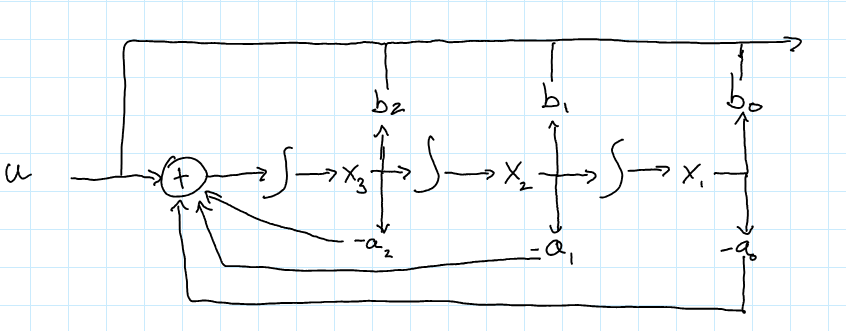
\includegraphics[width=0.55 \linewidth]{11-08-realization.png}
    \caption{Realization of problem 8}
    \label{fig:}
\end{figure}

\end{document}